\documentclass{article}\usepackage[]{graphicx}\usepackage[]{color}
% maxwidth is the original width if it is less than linewidth
% otherwise use linewidth (to make sure the graphics do not exceed the margin)
\makeatletter
\def\maxwidth{ %
  \ifdim\Gin@nat@width>\linewidth
    \linewidth
  \else
    \Gin@nat@width
  \fi
}
\makeatother

\definecolor{fgcolor}{rgb}{0.345, 0.345, 0.345}
\newcommand{\hlnum}[1]{\textcolor[rgb]{0.686,0.059,0.569}{#1}}%
\newcommand{\hlstr}[1]{\textcolor[rgb]{0.192,0.494,0.8}{#1}}%
\newcommand{\hlcom}[1]{\textcolor[rgb]{0.678,0.584,0.686}{\textit{#1}}}%
\newcommand{\hlopt}[1]{\textcolor[rgb]{0,0,0}{#1}}%
\newcommand{\hlstd}[1]{\textcolor[rgb]{0.345,0.345,0.345}{#1}}%
\newcommand{\hlkwa}[1]{\textcolor[rgb]{0.161,0.373,0.58}{\textbf{#1}}}%
\newcommand{\hlkwb}[1]{\textcolor[rgb]{0.69,0.353,0.396}{#1}}%
\newcommand{\hlkwc}[1]{\textcolor[rgb]{0.333,0.667,0.333}{#1}}%
\newcommand{\hlkwd}[1]{\textcolor[rgb]{0.737,0.353,0.396}{\textbf{#1}}}%
\let\hlipl\hlkwb

\usepackage{framed}
\makeatletter
\newenvironment{kframe}{%
 \def\at@end@of@kframe{}%
 \ifinner\ifhmode%
  \def\at@end@of@kframe{\end{minipage}}%
  \begin{minipage}{\columnwidth}%
 \fi\fi%
 \def\FrameCommand##1{\hskip\@totalleftmargin \hskip-\fboxsep
 \colorbox{shadecolor}{##1}\hskip-\fboxsep
     % There is no \\@totalrightmargin, so:
     \hskip-\linewidth \hskip-\@totalleftmargin \hskip\columnwidth}%
 \MakeFramed {\advance\hsize-\width
   \@totalleftmargin\z@ \linewidth\hsize
   \@setminipage}}%
 {\par\unskip\endMakeFramed%
 \at@end@of@kframe}
\makeatother

\definecolor{shadecolor}{rgb}{.97, .97, .97}
\definecolor{messagecolor}{rgb}{0, 0, 0}
\definecolor{warningcolor}{rgb}{1, 0, 1}
\definecolor{errorcolor}{rgb}{1, 0, 0}
\newenvironment{knitrout}{}{} % an empty environment to be redefined in TeX

\usepackage{alltt}
\IfFileExists{upquote.sty}{\usepackage{upquote}}{}
\begin{document}
By Ali Gharouni,
\begin{knitrout}
\definecolor{shadecolor}{rgb}{0.969, 0.969, 0.969}\color{fgcolor}\begin{kframe}
\begin{verbatim}
## [1] "2020-12-13 08:16:24 EST"
\end{verbatim}
\end{kframe}
\end{knitrout}
This is my a test for MacPan package.

\section{Install and Play}

\begin{knitrout}
\definecolor{shadecolor}{rgb}{0.969, 0.969, 0.969}\color{fgcolor}\begin{kframe}
\begin{alltt}
\hlcom{# install remotes package if necessary:}
\hlkwa{while} \hlstd{(}\hlopt{!}\hlkwd{require}\hlstd{(remotes)) \{}
    \hlkwd{install.packages}\hlstd{(}\hlstr{"remotes"}\hlstd{)}
\hlstd{\}}
\end{alltt}


{\ttfamily\noindent\itshape\color{messagecolor}{\#\# Loading required package: remotes}}\begin{alltt}
\hlcom{## install development version of bbmle:}
\hlkwa{if} \hlstd{(}\hlopt{!}\hlkwd{require}\hlstd{(}\hlstr{"bbmle"}\hlstd{)} \hlopt{||} \hlkwd{packageVersion}\hlstd{(}\hlstr{"bbmle"}\hlstd{)} \hlopt{<} \hlstr{"1.0.23.5"}\hlstd{) \{}
    \hlstd{remotes}\hlopt{::}\hlkwd{install_github}\hlstd{(}\hlstr{"bbolker/bbmle"}\hlstd{)}
\hlstd{\}}
\end{alltt}


{\ttfamily\noindent\itshape\color{messagecolor}{\#\# Loading required package: bbmle}}

{\ttfamily\noindent\itshape\color{messagecolor}{\#\# Loading required package: stats4}}\begin{alltt}
\hlcom{## install the target package and all its dependencies:}
\hlstd{remotes}\hlopt{::}\hlkwd{install_github}\hlstd{(}\hlstr{"bbolker/McMasterPandemic"}\hlstd{,}
                        \hlkwc{dependencies} \hlstd{=} \hlnum{TRUE}\hlstd{,}
                        \hlkwc{build_vignettes} \hlstd{=} \hlnum{TRUE}
\hlstd{)}
\end{alltt}


{\ttfamily\noindent\itshape\color{messagecolor}{\#\# Skipping install of 'McMasterPandemic' from a github remote, the SHA1 (54095dc4) has not changed since last install.\\\#\#\ \  Use `force = TRUE` to force installation}}\begin{alltt}
\hlkwd{library}\hlstd{(McMasterPandemic)}
\hlkwd{library}\hlstd{(ggplot2);} \hlkwd{theme_set}\hlstd{(}\hlkwd{theme_bw}\hlstd{())}
\hlkwd{library}\hlstd{(cowplot)}

\hlkwd{library}\hlstd{(directlabels)}
\hlkwd{library}\hlstd{(zoo)}
\end{alltt}


{\ttfamily\noindent\itshape\color{messagecolor}{\#\# \\\#\# Attaching package: 'zoo'}}

{\ttfamily\noindent\itshape\color{messagecolor}{\#\# The following objects are masked from 'package:base':\\\#\# \\\#\#\ \ \ \  as.Date, as.Date.numeric}}\begin{alltt}
\hlkwd{library}\hlstd{(tidyverse)}
\end{alltt}


{\ttfamily\noindent\itshape\color{messagecolor}{\#\# -- Attaching packages --------------------------------------- tidyverse 1.3.0 --}}

{\ttfamily\noindent\itshape\color{messagecolor}{\#\# v tibble\ \ 3.0.4\ \ \ \  v dplyr\ \  1.0.2\\\#\# v tidyr\ \  1.1.2\ \ \ \  v stringr 1.4.0\\\#\# v readr\ \  1.3.1\ \ \ \  v forcats 0.5.0\\\#\# v purrr\ \  0.3.4}}

{\ttfamily\noindent\itshape\color{messagecolor}{\#\# -- Conflicts ------------------------------------------ tidyverse\_conflicts() --\\\#\# x dplyr::filter() masks stats::filter()\\\#\# x dplyr::lag()\ \ \ \ masks stats::lag()\\\#\# x dplyr::slice()\ \ masks bbmle::slice()\\\#\# x tidyr::unpack() masks McMasterPandemic::unpack()}}\end{kframe}
\end{knitrout}


\begin{knitrout}
\definecolor{shadecolor}{rgb}{0.969, 0.969, 0.969}\color{fgcolor}\begin{kframe}
\begin{alltt}
\hlstd{params} \hlkwb{<-} \hlkwd{read_params}\hlstd{(}\hlstr{"ICU1.csv"}\hlstd{)}

\hlstd{knitr}\hlopt{::}\hlkwd{kable}\hlstd{(}\hlkwd{round}\hlstd{(}\hlkwd{t}\hlstd{(}\hlkwd{summary}\hlstd{(params)),}\hlnum{2}\hlstd{))}
\end{alltt}
\end{kframe}
\begin{tabular}{r|r|r|r|r}
\hline
r0 & R0 & Gbar & CFR\_gen & dbl\_time\\
\hline
0.23 & 6.52 & 12.19 & 0.04 & 3.04\\
\hline
\end{tabular}

\begin{kframe}\begin{alltt}
\hlstd{knitr}\hlopt{::}\hlkwd{kable}\hlstd{(}\hlkwd{round}\hlstd{(}\hlkwd{t}\hlstd{(}\hlkwd{get_R0}\hlstd{(params,} \hlkwc{components}\hlstd{=}\hlnum{TRUE}\hlstd{)),}\hlnum{2}\hlstd{))}
\end{alltt}
\end{kframe}
\begin{tabular}{r|r|r|r}
\hline
asymptomatic & pre-symptomatic & mild & severe\\
\hline
1.56 & 0.33 & 4.46 & 0.17\\
\hline
\end{tabular}


\end{knitrout}


\begin{knitrout}
\definecolor{shadecolor}{rgb}{0.969, 0.969, 0.969}\color{fgcolor}\begin{kframe}
\begin{alltt}
\hlcom{# A simple SIR model}
\hlkwd{library}\hlstd{(deSolve)}
\hlstd{unpack} \hlkwb{<-} \hlstd{McMasterPandemic}\hlopt{::}\hlstd{unpack}

\hlstd{sir.mod} \hlkwb{<-} \hlkwa{function}\hlstd{(}\hlkwc{time}\hlstd{,}\hlkwc{state}\hlstd{,}\hlkwc{params}\hlstd{)\{}
    \hlkwd{unpack}\hlstd{(}\hlkwd{as.list}\hlstd{(}\hlkwd{c}\hlstd{(state,params)))}
    \hlstd{dS.dt} \hlkwb{<-} \hlopt{-}\hlstd{beta}\hlopt{*}\hlstd{S}\hlopt{*}\hlstd{I}\hlopt{/}\hlstd{N0}
    \hlstd{dI.dt} \hlkwb{<-}  \hlstd{beta}\hlopt{*}\hlstd{S}\hlopt{*}\hlstd{I}\hlopt{/}\hlstd{N0}\hlopt{-}\hlstd{gamma}\hlopt{*}\hlstd{I}
    \hlstd{dR.dt} \hlkwb{<-}  \hlstd{gamma}\hlopt{*}\hlstd{I}
    \hlcom{# return the rate of change}
    \hlstd{dxdt} \hlkwb{<-} \hlkwd{c}\hlstd{(dS.dt,dI.dt,dR.dt)}
    \hlkwd{return}\hlstd{(}\hlkwd{list}\hlstd{(dxdt))}
\hlstd{\}}
\hlstd{sir.params} \hlkwb{<-} \hlkwd{c}\hlstd{(}\hlkwc{N0}\hlstd{=}\hlnum{10}\hlopt{^}\hlnum{6}\hlstd{,} \hlkwc{beta}\hlstd{=}\hlnum{0.5}\hlstd{,}\hlkwc{gamma}\hlstd{=}\hlnum{1}\hlopt{/}\hlnum{7}\hlstd{)}
\hlkwd{class}\hlstd{(sir.params)} \hlkwb{<-} \hlstr{"params_pansim"}
\hlcom{# Set the initial state}
\hlstd{sir.state_init} \hlkwb{<-} \hlkwd{c}\hlstd{(}\hlkwc{S}\hlstd{=sir.params[[}\hlstr{"N0"}\hlstd{]],}
                \hlkwc{I}\hlstd{=}\hlnum{1}\hlstd{,}
                \hlkwc{R}\hlstd{=}\hlnum{0}\hlstd{)}
\hlcom{##set the number of days for SIR simulation as simulation time of MacPan}
\hlstd{startdate} \hlkwb{<-} \hlkwd{as.Date}\hlstd{(}\hlstr{"01-03-2020"}\hlstd{)}
\hlstd{enddate} \hlkwb{<-} \hlkwd{as.Date}\hlstd{(}\hlstr{"01-09-2020"}\hlstd{)}
\hlstd{d} \hlkwb{<-} \hlkwd{seq}\hlstd{(}\hlnum{0}\hlstd{,}\hlkwd{as.numeric}\hlstd{(enddate}\hlopt{-}\hlstd{startdate),}\hlkwc{by}\hlstd{=}\hlnum{1}\hlstd{)}

\hlstd{sir.R0} \hlkwb{<-} \hlstd{sir.params[[}\hlstr{"beta"}\hlstd{]]}\hlopt{/}\hlstd{sir.params[[}\hlstr{"gamma"}\hlstd{]]}

\hlstd{sir.out} \hlkwb{<-} \hlkwd{as.data.frame}\hlstd{(}
  \hlkwd{ode}\hlstd{(}
    \hlkwc{func}\hlstd{=sir.mod,}
    \hlkwc{y}\hlstd{=sir.state_init,}
    \hlkwc{times}\hlstd{= d,}
    \hlkwc{parms}\hlstd{=}\hlkwd{update}\hlstd{(sir.params)}
    \hlstd{))}

\hlstd{sir.out2} \hlkwb{<-} \hlstd{sir.out} \hlopt
  \hlkwd{pivot_longer}\hlstd{(}\hlkwd{c}\hlstd{(S,I,R),} \hlkwc{names_to} \hlstd{=} \hlstr{"compartment"}\hlstd{,} \hlkwc{values_to} \hlstd{=} \hlstr{"value"}\hlstd{)}

\hlstd{gg1} \hlkwb{<-} \hlstd{(}\hlkwd{ggplot}\hlstd{(}\hlkwc{data}\hlstd{=sir.out2,} \hlkwd{aes}\hlstd{(}\hlkwc{x}\hlstd{=time,}\hlkwc{y}\hlstd{=value,}\hlkwc{col}\hlstd{=compartment))}
    \hlopt{+} \hlkwd{geom_line}\hlstd{()}
    \hlcom{# + scale_y_log10(limits=c(0.1,sir.params[["N0"]]))}
\hlstd{)}
\hlkwd{direct.label}\hlstd{(gg1,}\hlstr{"last.bumpup"}\hlstd{)}
\end{alltt}
\end{kframe}
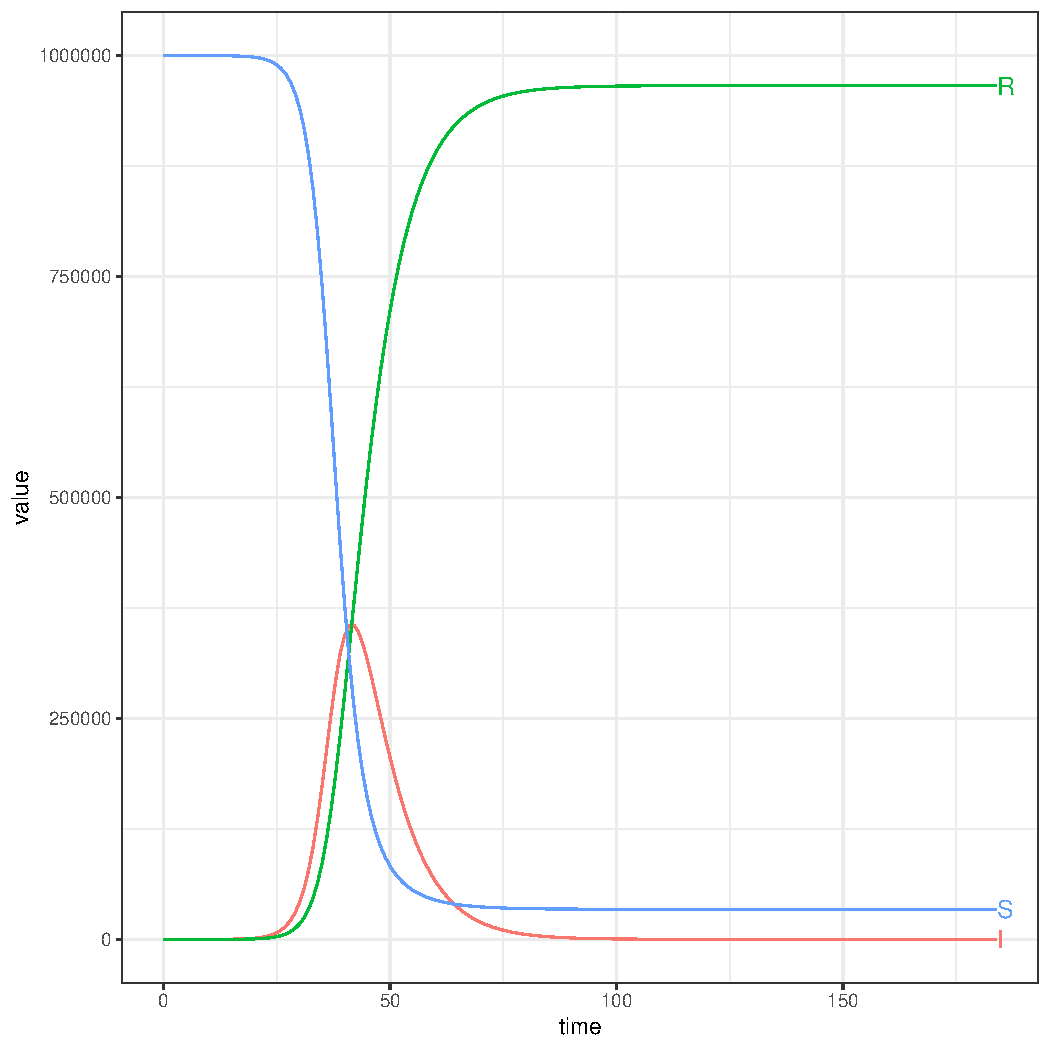
\includegraphics[width=\maxwidth]{figure/Ali:SIR_-1} 

\end{knitrout}


\begin{knitrout}
\definecolor{shadecolor}{rgb}{0.969, 0.969, 0.969}\color{fgcolor}\begin{kframe}
\begin{alltt}
\hlcom{## update MacPan's params according to the SIR params}
\hlcom{##}
\hlstd{big_rate} \hlkwb{<-} \hlnum{20}
\hlstd{params} \hlkwb{<-} \hlkwd{update}\hlstd{(params,} \hlkwd{c}\hlstd{(}\hlkwc{beta0}\hlstd{=sir.params[[}\hlstr{"beta"}\hlstd{]],}
                           \hlkwc{alpha}\hlstd{=}\hlnum{0}\hlstd{,} \hlcom{## no asymptomatic}
                           \hlkwc{sigma}\hlstd{=big_rate,} \hlcom{## very short latent period}
                           \hlcom{## would like this to -> Inf but can't}
                           \hlkwc{gamma_a}\hlstd{=}\hlnum{0}\hlstd{,}
                           \hlkwc{mu}\hlstd{=}\hlnum{1}\hlstd{,}  \hlcom{## all cases mild}
                           \hlkwc{gamma_m}\hlstd{=sir.params[[}\hlstr{"gamma"}\hlstd{]],}
                           \hlkwc{gamma_s}\hlstd{=}\hlnum{0}\hlstd{,}
                           \hlcom{## try to skip presymptomatic period}
                           \hlkwc{gamma_p}\hlstd{=big_rate}
                           \hlstd{))}

\hlstd{pp} \hlkwb{<-} \hlstd{params}
\hlcom{## pp <- fix_pars(params, target = c(R0 = sir.R0)) #not sure if I need to update Gbar=6?}
\hlstd{state} \hlkwb{<-} \hlkwd{make_state}\hlstd{(}\hlkwc{params}\hlstd{=pp)}
\hlstd{state[]} \hlkwb{<-} \hlnum{0}
\hlstd{state[[}\hlstr{"S"}\hlstd{]]} \hlkwb{<-} \hlnum{1e6}
\hlstd{state[[}\hlstr{"Im"}\hlstd{]]} \hlkwb{<-} \hlnum{1}

\hlkwd{summary}\hlstd{(pp)}
\end{alltt}


{\ttfamily\noindent\color{warningcolor}{\#\# Warning in log(r\_last/r\_nextlast): NaNs produced}}\begin{verbatim}
##       r0       R0     Gbar  CFR_gen dbl_time 
##      NaN      NaN      NaN        0      NaN
\end{verbatim}
\begin{alltt}
\hlstd{sim0} \hlkwb{<-} \hlkwd{run_sim}\hlstd{(pp,state,}
                \hlkwc{start_date}\hlstd{=startdate,}
                \hlkwc{end_date}\hlstd{=enddate,}
                \hlkwc{use_ode}\hlstd{=}\hlnum{TRUE}\hlstd{)}

\hlstd{gg0} \hlkwb{<-} \hlstd{(}\hlkwd{ggplot}\hlstd{(sim0,}\hlkwd{aes}\hlstd{(}\hlkwc{x}\hlstd{=date))}
\hlopt{+} \hlkwd{geom_point}\hlstd{(}\hlkwd{aes}\hlstd{(}\hlkwc{y}\hlstd{=incidence))}
\hlstd{)}
\hlkwd{print}\hlstd{(gg0)}
\end{alltt}
\end{kframe}
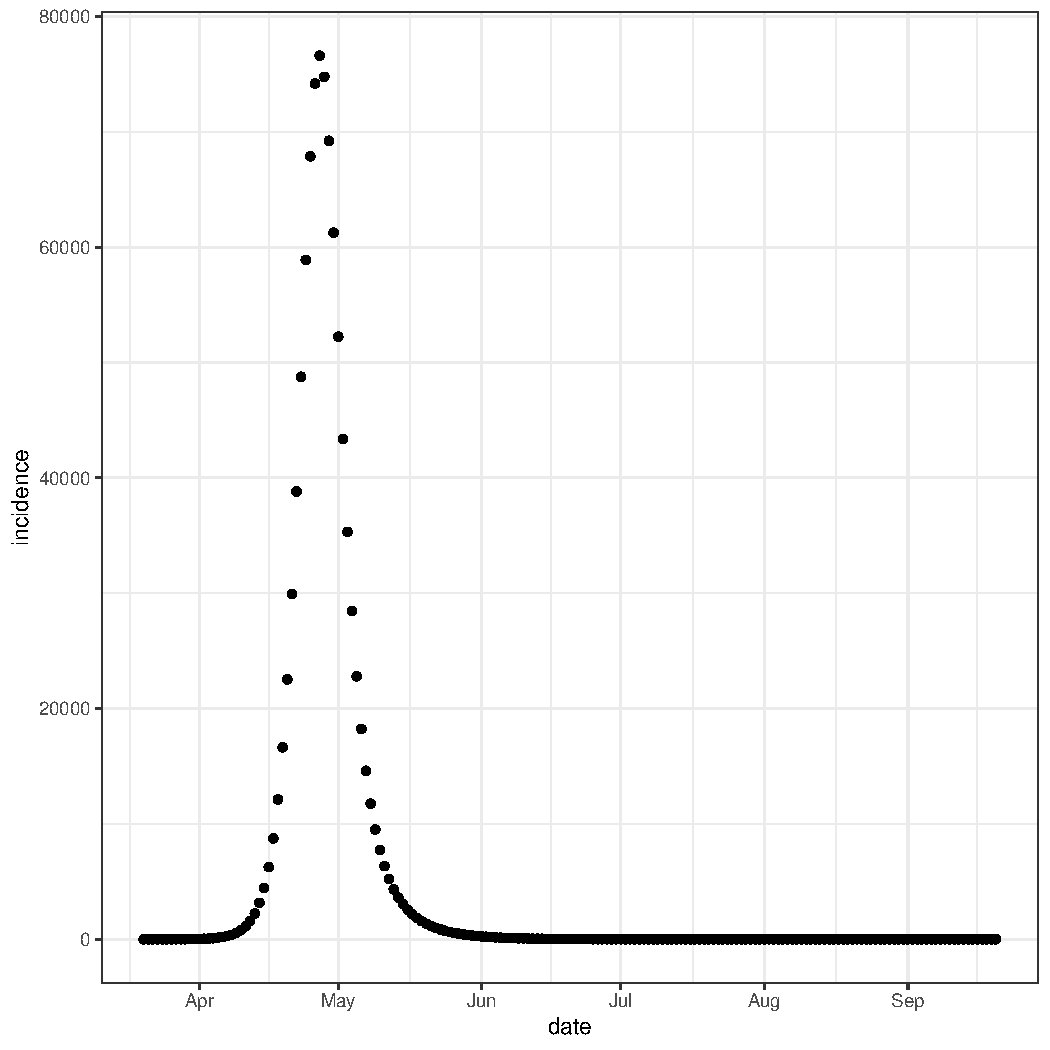
\includegraphics[width=\maxwidth]{figure/Try_MacPan_to_recover_the_SIR_result-1} 
\begin{kframe}\begin{alltt}
\hlcom{# combining the SIR and MacPan results also calculating incidences fr the SIR model}
\hlstd{sim_combined} \hlkwb{<-} \hlstd{sim0} \hlopt \hlkwd{mutate}\hlstd{(}\hlkwc{sir.S}\hlstd{=sir.out[[}\hlstr{"S"}\hlstd{]],}
                                \hlkwc{sir.I}\hlstd{=sir.out[[}\hlstr{"I"}\hlstd{]],}
                                \hlkwc{sir.S}\hlstd{=sir.out[[}\hlstr{"R"}\hlstd{]],}
                                \hlkwc{sir.incidence}\hlstd{=sir.params[[}\hlstr{"beta"}\hlstd{]]}\hlopt{*}\hlstd{sir.out[[}\hlstr{"S"}\hlstd{]]}\hlopt{*}\hlstd{sir.out[[}\hlstr{"I"}\hlstd{]])}

\hlstd{gg01} \hlkwb{<-} \hlstd{(}\hlkwd{ggplot}\hlstd{(sim_combined,}\hlkwd{aes}\hlstd{(}\hlkwc{x}\hlstd{=date))}
\hlopt{+} \hlkwd{geom_point}\hlstd{(}\hlkwd{aes}\hlstd{(}\hlkwc{y}\hlstd{=I))}
\hlopt{+} \hlkwd{geom_line}\hlstd{(}\hlkwd{aes}\hlstd{(}\hlkwc{y}\hlstd{=sir.I),} \hlkwc{color}\hlstd{=}\hlstr{'red'}\hlstd{)}
\hlstd{)}
\hlkwd{print}\hlstd{(gg01)}
\end{alltt}
\end{kframe}
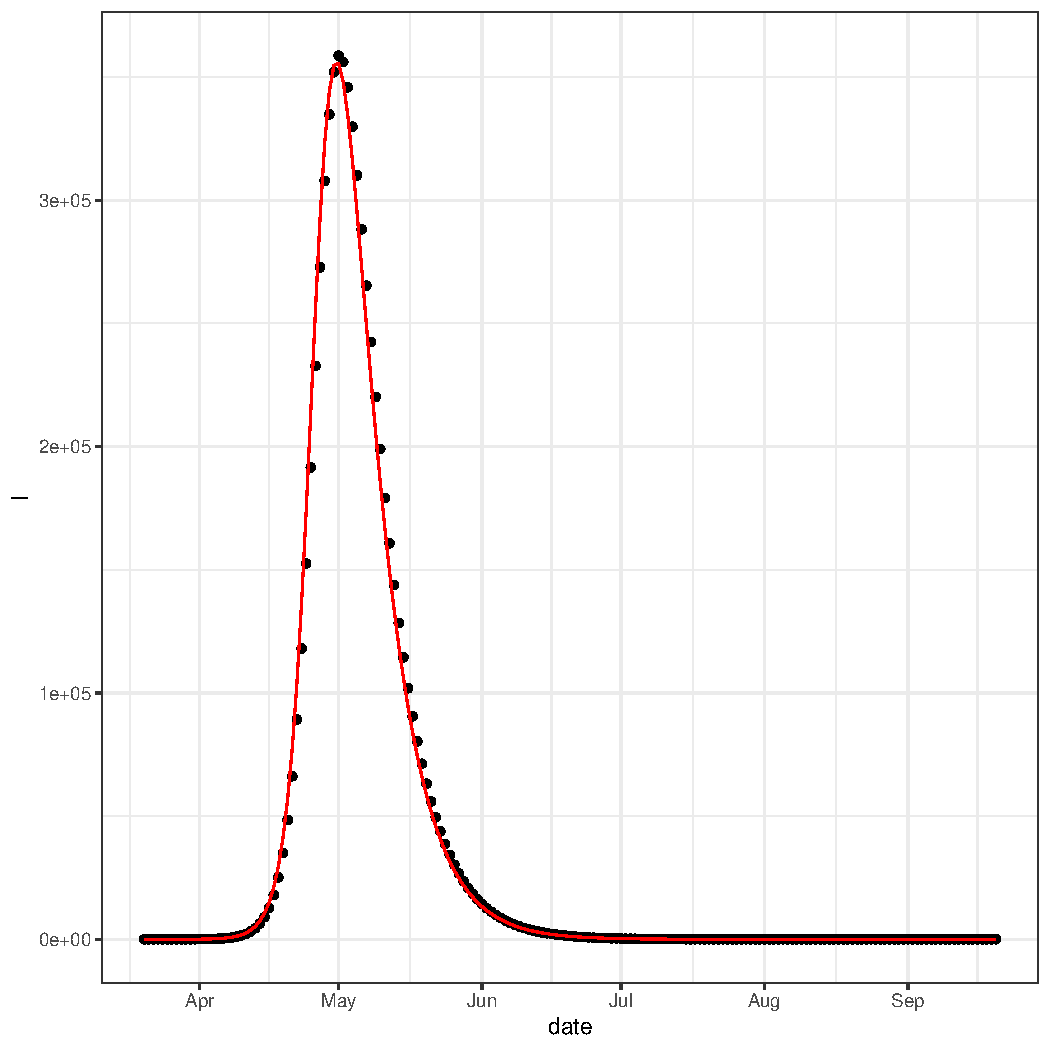
\includegraphics[width=\maxwidth]{figure/Try_MacPan_to_recover_the_SIR_result-2} 
\begin{kframe}\begin{alltt}
\hlkwd{print}\hlstd{(gg01} \hlopt{+} \hlkwd{scale_y_log10}\hlstd{())}
\end{alltt}
\end{kframe}
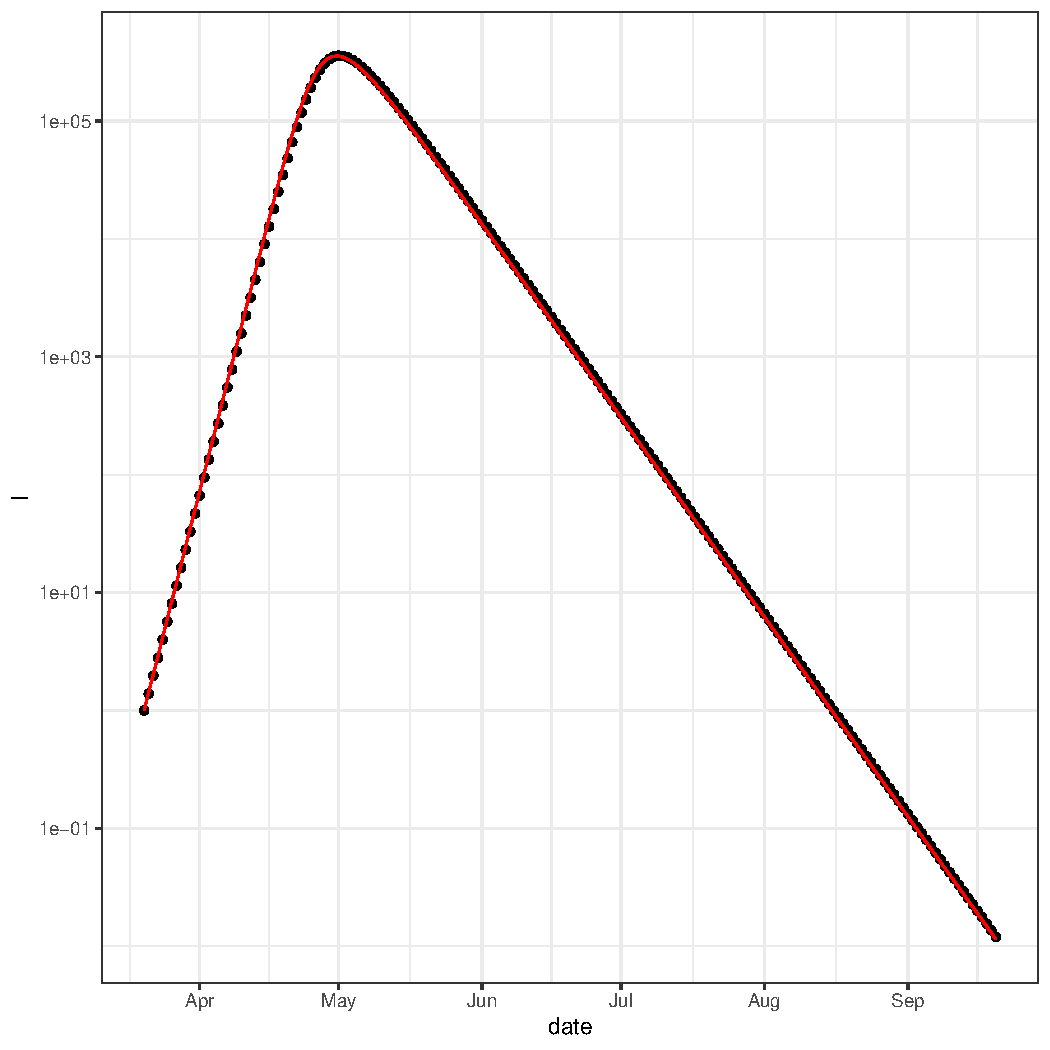
\includegraphics[width=\maxwidth]{figure/Try_MacPan_to_recover_the_SIR_result-3} 

\end{knitrout}




\end{document}
